\documentclass[draft=false
              ,paper=a4
              ,twoside=false
              ,fontsize=11pt
              ,headsepline
              ,BCOR10mm
              ,DIV11
              ]{scrbook}
\usepackage[ngerman,english]{babel}
\usepackage[T1]{fontenc}
\usepackage[utf8]{inputenc}
\usepackage{libertine}
\usepackage{pifont}
\usepackage{microtype}
\usepackage{textcomp}
\usepackage[german,refpage]{nomencl}
\usepackage{setspace}
\usepackage{makeidx}
\usepackage{listings}
\usepackage{natbib}
\usepackage[ngerman,colorlinks=true]{hyperref}
\usepackage{soul}
\usepackage{hawstyle}

%% define some colors
\colorlet{BackgroundColor}{gray!20}
\colorlet{KeywordColor}{blue}
\colorlet{CommentColor}{black!60}
%% for tables
\colorlet{HeadColor}{gray!60}
\colorlet{Color1}{blue!10}
\colorlet{Color2}{white}

%% configure colors
\HAWifprinter{
  \colorlet{BackgroundColor}{gray!20}
  \colorlet{KeywordColor}{black}
  \colorlet{CommentColor}{gray}
  % for tables
  \colorlet{HeadColor}{gray!60}
  \colorlet{Color1}{gray!40}
  \colorlet{Color2}{white}
}{}
\lstset{%
  numbers=left,
  numberstyle=\tiny,
  stepnumber=1,
  numbersep=5pt,
  basicstyle=\ttfamily\small,
  keywordstyle=\color{KeywordColor}\bfseries,
  identifierstyle=\color{black},
  commentstyle=\color{CommentColor},
  backgroundcolor=\color{BackgroundColor},
  captionpos=b,
  fontadjust=true
}
\lstset{escapeinside={(*@}{@*)}, % used to enter latex code inside listings
        morekeywords={uint32_t, int32_t}
}
\ifpdfoutput{
  \hypersetup{bookmarksopen=false,bookmarksnumbered,linktocpage}
}{}

%% more fancy C++
\DeclareRobustCommand{\cxx}{C\raisebox{0.25ex}{{\scriptsize +\kern-0.25ex +}}}

\lstdefinelanguage{clojure}%
{morekeywords={*,*1,*2,*3,*agent*,*allow-unresolved-vars*,*assert*,*clojure-version*,*command-line-args*,%
*compile-files*,*compile-path*,*e,*err*,*file*,*flush-on-newline*,*in*,*macro-meta*,%
*math-context*,*ns*,*out*,*print-dup*,*print-length*,*print-level*,*print-meta*,*print-readably*,%
*read-eval*,*source-path*,*use-context-classloader*,*warn-on-reflection*,+,-,->,->>,..,/,:else,%
<,<=,=,==,>,>=,@,accessor,aclone,add-classpath,add-watch,agent,agent-errors,aget,alength,alias,%
all-ns,alter,alter-meta!,alter-var-root,amap,ancestors,and,apply,areduce,array-map,aset,%
aset-boolean,aset-byte,aset-char,aset-double,aset-float,aset-int,aset-long,aset-short,assert,%
assoc,assoc!,assoc-in,associative?,atom,await,await-for,await1,bases,bean,bigdec,bigint,binding,%
bit-and,bit-and-not,bit-clear,bit-flip,bit-not,bit-or,bit-set,bit-shift-left,bit-shift-right,%
bit-test,bit-xor,boolean,boolean-array,booleans,bound-fn,bound-fn*,butlast,byte,byte-array,%
bytes,cast,char,char-array,char-escape-string,char-name-string,char?,chars,chunk,chunk-append,%
chunk-buffer,chunk-cons,chunk-first,chunk-next,chunk-rest,chunked-seq?,class,class?,%
clear-agent-errors,clojure-version,coll?,comment,commute,comp,comparator,compare,compare-and-set!,%
compile,complement,concat,cond,condp,conj,conj!,cons,constantly,construct-proxy,contains?,count,%
counted?,create-ns,create-struct,cycle,dec,decimal?,declare,def,definline,defmacro,defmethod,%
defmulti,defn,defn-,defonce,defprotocol,defstruct,deftype,delay,delay?,deliver,deref,derive,%
descendants,destructure,disj,disj!,dissoc,dissoc!,distinct,distinct?,do,do-template,doall,doc,%
dorun,doseq,dosync,dotimes,doto,double,double-array,doubles,drop,drop-last,drop-while,empty,empty?,%
ensure,enumeration-seq,eval,even?,every?,false,false?,ffirst,file-seq,filter,finally,find,find-doc,%
find-ns,find-var,first,float,float-array,float?,floats,flush,fn,fn?,fnext,for,force,format,future,%
future-call,future-cancel,future-cancelled?,future-done?,future?,gen-class,gen-interface,gensym,%
get,get-in,get-method,get-proxy-class,get-thread-bindings,get-validator,hash,hash-map,hash-set,%
identical?,identity,if,if-let,if-not,ifn?,import,in-ns,inc,init-proxy,instance?,int,int-array,%
integer?,interleave,intern,interpose,into,into-array,ints,io!,isa?,iterate,iterator-seq,juxt,%
key,keys,keyword,keyword?,last,lazy-cat,lazy-seq,let,letfn,line-seq,list,list*,list?,load,load-file,%
load-reader,load-string,loaded-libs,locking,long,long-array,longs,loop,macroexpand,macroexpand-1,%
make-array,make-hierarchy,map,map?,mapcat,max,max-key,memfn,memoize,merge,merge-with,meta,%
method-sig,methods,min,min-key,mod,monitor-enter,monitor-exit,name,namespace,neg?,new,newline,%
next,nfirst,nil,nil?,nnext,not,not-any?,not-empty,not-every?,not=,ns,ns-aliases,ns-imports,%
ns-interns,ns-map,ns-name,ns-publics,ns-refers,ns-resolve,ns-unalias,ns-unmap,nth,nthnext,num,%
number?,odd?,or,parents,partial,partition,pcalls,peek,persistent!,pmap,pop,pop!,pop-thread-bindings,%
pos?,pr,pr-str,prefer-method,prefers,primitives-classnames,print,print-ctor,print-doc,print-dup,%
print-method,print-namespace-doc,print-simple,print-special-doc,print-str,printf,println,println-str,%
prn,prn-str,promise,proxy,proxy-call-with-super,proxy-mappings,proxy-name,proxy-super,%
push-thread-bindings,pvalues,quot,rand,rand-int,range,ratio?,rational?,rationalize,re-find,%
re-groups,re-matcher,re-matches,re-pattern,re-seq,read,read-line,read-string,recur,reduce,ref,%
ref-history-count,ref-max-history,ref-min-history,ref-set,refer,refer-clojure,reify,%
release-pending-sends,rem,remove,remove-method,remove-ns,remove-watch,repeat,repeatedly,%
replace,replicate,require,reset!,reset-meta!,resolve,rest,resultset-seq,reverse,reversible?,%
rseq,rsubseq,second,select-keys,send,send-off,seq,seq?,seque,sequence,sequential?,set,set!,%
set-validator!,set?,short,short-array,shorts,shutdown-agents,slurp,some,sort,sort-by,sorted-map,%
sorted-map-by,sorted-set,sorted-set-by,sorted?,special-form-anchor,special-symbol?,split-at,%
split-with,str,stream?,string?,struct,struct-map,subs,subseq,subvec,supers,swap!,symbol,symbol?,%
sync,syntax-symbol-anchor,take,take-last,take-nth,take-while,test,the-ns,throw,time,to-array,%
to-array-2d,trampoline,transient,tree-seq,true,true?,try,type,unchecked-add,unchecked-dec,%
unchecked-divide,unchecked-inc,unchecked-multiply,unchecked-negate,unchecked-remainder,%
unchecked-subtract,underive,unquote,unquote-splicing,update-in,update-proxy,use,val,vals,%
var,var-get,var-set,var?,vary-meta,vec,vector,vector?,when,when-first,when-let,when-not,%
while,with-bindings,with-bindings*,with-in-str,with-loading-context,with-local-vars,%
with-meta,with-open,with-out-str,with-precision,xml-seq,zero?,zipmap
},%
   sensitive,% ???
   alsodigit=-,%
   morecomment=[l];,%
   morestring=[b]"%
  }[keywords,comments,strings]%

\lstset{language=clojure}

\clubpenalty=10000
\widowpenalty=10000
\displaywidowpenalty=10000

% unknown hyphenations
\hyphenation{
}

%% recalculate text area
\typearea[current]{last}

%% no indentation at paragraphs
\setlength\parindent{0pt}
\setlength\parskip{\medskipamount}

\makeindex
\makenomenclature

\begin{document}
\selectlanguage{ngerman}

%%%%%
%% customize (see readme.pdf for supported values)
\HAWThesisProperties{Author={Daniel Schruhl}
                    ,Title={Entwurf und Implementierung einer STDMA Station}
                    ,EnglishTitle={Design and implementation of an STDMA station}
                    ,ThesisType={Referat}
                    ,ExaminationType={Referat eingereicht im Rahmen der Vorlesung Verteilte Systeme}
                    ,DegreeProgramme={Angewandte Informatik (AI)}
                    ,ThesisExperts={Prof. Dr. C. Klauck}
                    ,ReleaseDate={31. Mai 2017}
                  }

%% title
\frontmatter

%% output title page
\maketitle

\onehalfspacing

%% add abstract pages
%% note: this is one command on multiple lines
\HAWAbstractPage
%% German abstract
{STDMA, Verteilte Systeme, Clojure}%
{Umsetzung einer STDMA Station auf IP-Multicast Socket Basis}%
%% English abstract
{STDMA, Distributed Systems, Clojure}%
{Implementation of an STDMA Station via IP-Multicast Sockets}%

\newpage
\singlespacing

\tableofcontents
\newpage
%% enable if these lists should be shown on their own page
%%\listoftables
%%\listoffigures
%\lstlistoflistings

%% main
\mainmatter
\onehalfspacing
%% write to the log/stdout
\typeout{===== File: chapter 1}
%% include chapter file (chapter1.tex)
%%\include{chapter1}

\chapter{Einführung und Ziele}
In verteilten Systemen werden oft Nachrichten unter verschiedenen Teilnehmern eines Netzes ausgetauscht. Dabei sind diese Teilnehmer oft nur durch ein Medium miteinander verbunden. Dieses eine Medium muss dann mehrere Teilnehmer unterstützen können.

Um dieses Problem zu lösen soll ein Softwareprodukt erstellt werden, das eine Station darstellt, die auf einem Medium Nachrichten empfangen und senden kann.

Dabei sollen mehrere Stationen auf einem Medium Nachrichten verschicken und senden. Das geschieht, indem das Medium in feste Frames aufgeteilt wird und jeder Frame eine feste Anzahl an Slots hat, in dem aus allen teilnehmenden Stationen immer nur eine in ihrem zugeteilten Slot Senden darf. Das Medium wird hierbei im Betracht der Zeit aufgeteilt. Diese Aufteilung (Multiplexing) wird auch time-division multiple access (TDMA) genannt.
In diesem Fall sollen die Stationen selber untereinander ihre Slots zum Senden verwalten und untereinander gleichmäßig aufteilen.
Das wird auch Self-organized time-division multiple access (STDMA) genannt.

\section{Randbedingungen}
Das zu verwendende Medium ist ein Socket, der per IP Multicast Nachrichtenpakete (Datagrams) an mehrere Klienten austeilen kann. Die TTL der Multicast-Pakete ist auf 1 zu setzen, um unnötige Netzlasten und Netzstörungen zu vermeiden.

Die Frames haben eine Länge von einer Sekunde. Ein Frame hat 25 Slots. Diese sind von 1 bis 25 nummeriert. Die Frames sind in
Sekunden seit dem 1.1.1970, 00:00 Uhr nummeriert.

\begin{figure}[h]
\centering
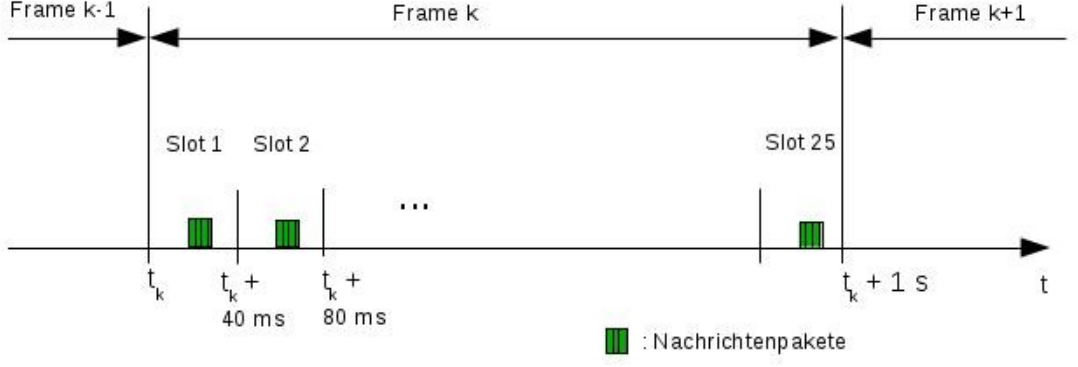
\includegraphics[width=\textwidth]{frame-structure.png}
\caption[frame-structure]{Aufteilung des Mediums in Frames und Slots, Quelle: \cite{exercise}}
\label{fig:frame-structure}
\end{figure}

Jede Station darf nur einmal pro Frame senden. Das muss in der Mitte ihres zugeteilten Slots passieren.

Die Vergabe der Slots soll ohne zentrale Vergabeinstanz geschehen. Das geschieht, indem jedes Nachrichtenpaket ein Datenfeld enthält, in das die sendende Station die Nummer ihres Slots einträgt, die sie für den nächsten Frame zum Senden verwendet.
Das bedeutet also, dass durch das Lesen der Nachrichtenpakete in einem Frame bestimmt werden kann, welche Slots im nächsten Frame frei sind.

Ein Nachrichtenpaket hat folgende Struktur:
\begin{itemize}
	\item Byte 0: Stationsklasse ('A' oder 'B')
	\item Byte 1 – 24: Nutzdaten. (Darin Byte 1 – 10: Name der sendenden Station.)
	\item Byte 25: Nummer des Slots, in dem die Station im nächsten Frame senden wird.
	\item Byte 26 – 33: Zeitpunkt, zu dem dieses Paket gesendet wurde. Einheit: Millisekunden seit dem 1.1.1970 als 8-Byte Integer, Big Endian.
\end{itemize}

Gesamtlänge: 34 Bytes

Stationen haben dabei eine Unterteilung in Klasse A und B. Diese Klassen werden für eine Synchronisierung der Zeit verwendet. Generell wird die UTC Zeit verwendet. Die Uhr einer Station kann einen anfänglichen Offset haben. Die Stationen synchronisieren dann untereinander im Laufe der Teilnahme am Netz ihre Uhren untereinander, so dass der Offset sich verändern kann.

Klasse A Uhren gelten als hinreichend genau und als Referenz zur Synchronisation. Klasse B und Klasse A Stationen können dann anhand anderer empfangen Nachrichtenpakete von Klasse A Stationen ihren Offset verändern. Dabei wird die Sendezeit und die Klasse innerhalb eines Nachrichtenpaketes verwendet.

Bei Kollisionen sollen die betroffenen Nachrichtenpakete als nicht empfangen betrachtet werden. Ein kollisionsfreier Betrieb mit maximal 25 Stationen muss nach endlicher Zeit erreicht werden und darf nicht wieder verlassen werden.

Das Produkt soll über die Kommandozeile gestartet werden können. Dabei müssen folgende Parameter mit übergeben werden können:
\begin{itemize}
	\item Interfacename des Kommunikationsendpunktes
	\item Adresse der Multicast Gruppe, Klasse D IP-Adresse
	\item Port des Sockets
	\item Stationsklasse, A oder B
	\item Anfänglicher UTC Offset
\end{itemize}
Als Datenquelle für die Nutzdaten soll das STDIN des Produktes verwendet werden, um der Station neue Nutzdaten zukommen zu lassen.

\section{Kontextabgrezung}
Das Produkt muss auch in einer ssh-Sitzung auf einem anderen Rechner gestartet werden können. Es muss auf Rechnern mit Linux Betriebssystem lauffähig sein.

\chapter{Gesamtsystem}
Das Produkt ist in Clojure (v1.9) umgesetzt worden. Clojure ist eine funktionale Programmiersprache, die auf der JVM läuft. Dabei ist eine interoperabilität mit Java möglich. Das erleichtert den Umgang mit Sockets, da der Umgang mit diesen in Java gut dokumentiert und verwendbar ist. Außerdem hat Clojure im Vergleich mit Erlang einige andere Vorteile wie lazily evaluated Sequences oder eine bessere Testumgebung.

Funktionale Programmiersprachen haben den Vorteil in verteilten Systemen, das die Ergebnisse von Funktionen bei gleichen Parametern immer gleich sind. Diese Immutability von Daten hat den Vorteil, das nebenläufige Prozesse dadurch keine Datensynchronisation machen müssen. Dadurch wird eine erhöhte Threadsicherheit erreicht.

\section{Architekturüberblick}
Das System ist in drei Pakete aufgeteilt, die jeweils aus verschiedenen Komponenten bestehen.
Die Pakete sind die Business Logik (Basis Paket), die Verbindungs Logik (Network Paket) und die Daten Verbindungs Logik (Data-Links Paket).

Das Paket mit der Business Logik enthält die Stations Komponente, die Uhren Komponente und den Haupteinstiegspunkt des Systems, das alle Komponenten zusammen baut. Hier sind die fachlichen Logiken, die das Verhalten der Station beeinflussen definiert.

Das Paket mit der Verbindungslogik enthält die Verbindungs Komponente und die Datagram Komponente. Hier werden alle verbindungsrelevanten Informationen verarbeitet. Dazu gehört der Aufbau und der Abbau und das Versenden und Verschicken von Nachrichtenpaketen auf Netzebene (Datagramme).

Das Daten Verbinungs Paket beinhaltet die Payload Source Komponente und die Message Writer Komponente. Dieses Paket ist für die Datensenke und Datenquelle zuständig. Sie Laufen Nebenläufig zu den anderen Komponenten, damit Sie diese nicht blockieren und so die fachliche Aufgabe des Gesamtsystems isoliert davon arbeiten kann.

\begin{figure}[h]
\centering
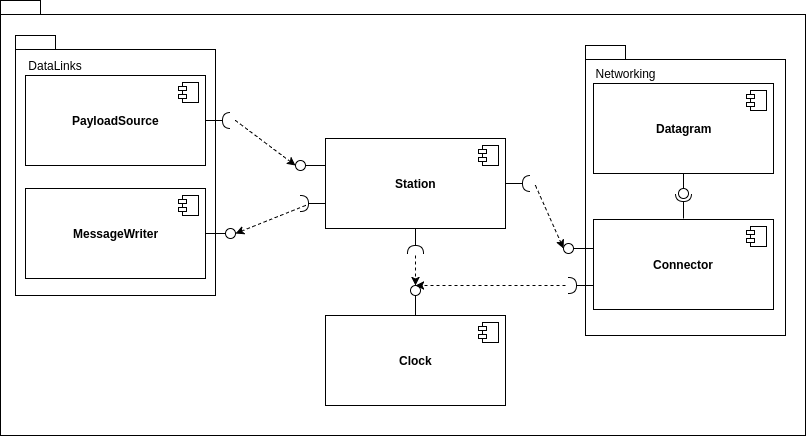
\includegraphics[width=\textwidth]{component-diagram.png}
\caption[component-diagram]{Komponentendiagramm des Gesamtsystems}
\label{fig:component-diagram}
\end{figure}

\begin{figure}[h]
\centering
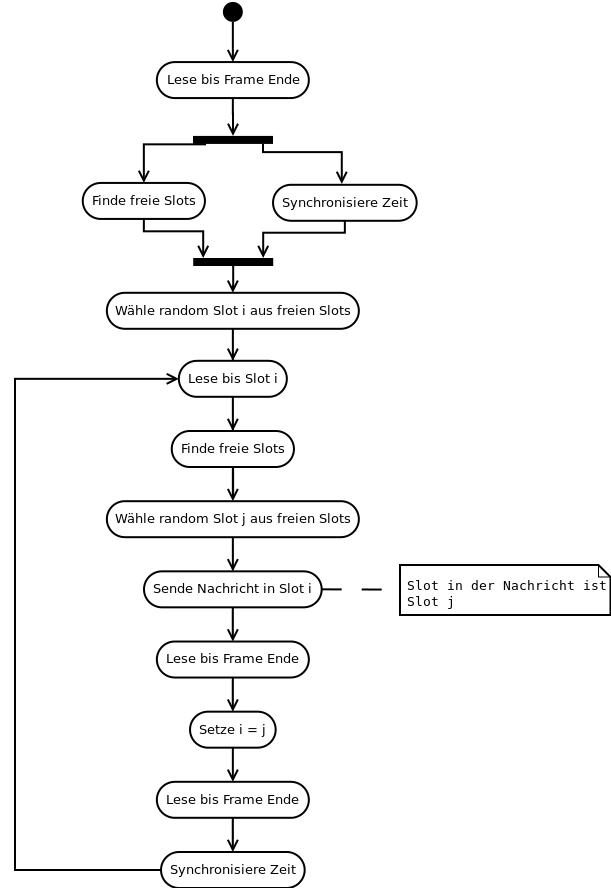
\includegraphics[width=0.8\textwidth]{activity-diagram.png}
\caption[activity-diagram]{Aktivitätendiagramm der Nachrichtenbehandlung im Gesamtsystem}
\label{fig:component-diagram}
\end{figure}

\begin{figure}[h]
\centering
\includegraphics[width=0.8\textwidth]{sequence-diagram.png}
\caption[sequence-diagram]{Sequenzdiagramm der Nachrichtenbehandlung im Gesamtsystem}
\label{fig:sequence-diagram}
\end{figure}

\section{Konfigurationsparameter}
Es existiert eine Konfigurationsdatei (./resources/default.edn), die folgende Parameter bestimmt:
\begin{itemize}
	\item Anzahl der slots
	\item Länge eines Frames in ms
	\item Länge eines Nachrichtenpaketes
	\item Länge der Nutznachricht
	\item Datei für die Datensenke
\end{itemize}

\section{Benutzungsschnittstellen}
Das System wird als .jar über die Kommandozeile gestartet mit folgenden Parameter (in Reihenfolge):
\begin{itemize}
	\item Interfacename 
	\item Multicastadresse
	\item Port
	\item Stationsklasse
	\item Initialer UTC Offset
\end{itemize}

\chapter{Subsysteme und Komponenten}
\section{Datagram}
\subsection{Aufgabe und Verantwortung}
Das Datagram Modul ist dafür verantwortlich aus vorhanden Nachrichten Byte Pakete zu erstellen und diese wieder in Nachrichten zurück zu konvertieren.

\subsection{Schnittstelle}
\begin{lstlisting}
; Prueft ob uebergebene Bytes nicht leer sind
Bytes -> Boolean
byte-array-empty?(bytes-array)

; Konvertiert uebergebene Bytes in ein Nachricht
Bytes -> Nachricht
datagram->message(bytes-array)

; Kodiert uebergebene Nachricht in ein Bytes
Nachricht -> Bytes
message->datagram(message)
\end{lstlisting}
Eine Nachricht ist eine Map folgender Gestalt:
\begin{lstlisting}
{:station-class   String
 :station-name    String
 :payload-content String
 :payload         String
 :slot            Nummer
 :send-time       Nummer}
\end{lstlisting}

\subsection{Entwurfsentscheidungen}
Nutznachrichten werden in ihrer Zeichenketten Form als UTF-8 konvertiert behandelt. Die Stationsklasse wird in Byte der jeweiligen String Repräsentation des Klassennamen konvertiert ('A' oder 'B').

Die Zeitstempel in den Nachrichten werden als Big Endian Bytes behandelt (eventuelles Zero Padding ist links).

\section{Connector}
\subsection{Aufgabe und Verantwortung}
Der Connector abstrahiert die Netzwerkverbindung, die per Multicast Sockets umgesetzt wurde. Über den Connector werden Nachrichten verschickt und empfangen. Das Verschicken und Empfangen ist mit einer Kollisionserkennung ausgestattet, so dass falsche Nachrichtenpakete verworfen werden.

Der Connector versendet Nachrichten und konvertiert diese in Nachrichtenpakete (Bytes). Beim Lesen werden Nachrichtenpakete (Bytes) eingelesen und als konvertierte Nachrichten zurückgegeben.

\subsection{Schnittstelle}
\begin{lstlisting}
; Startet den Connector und verbindet den Socket
Map -> Komponente
new-connector(config)

; Sendet eine Nachricht, wenn das Senden Kollisionsfrei ist
(Komponente, Nachricht) -> Boolean
send-message-collision-safe?(connector, message)

; Liest Nachrichten bis zum Ablauf des Timeouts
(Komponente, Nummer) -> Bytes
read-message-with-collision-detection(connector, timeout) 
\end{lstlisting}

Eine Komponente ist eine Map, die den State und die Konfiguration der Komponente enthalten in jeweils wieder einer Map.
\begin{lstlisting}
Map -> Map
{:config             Map
 :socket-connection  Map}
\end{lstlisting}

\subsection{Entwurfsentscheidungen}
Der Connector hat einen State, der seine Socketverbindung und Informationen zu dieser beinhaltet. Dazu gehört die IP-Adresse, der Port und das Interface.

Der Connector verbindet seinen Socket beim Start und tritt der angegebenen Multicast Gruppe bei. Beim Herunterfahren, baut er die Verbindung wieder ab.

Der Sendevorgang im Connector liest vor dem Zeitpunkt des Sendens (20 ms nach Aufruf) Nachrichten, um zu überprüfen, ob der geplante Sendevorgang überhaupt gültig ist. Wenn Nachrichten vor dem Senden empfangen wurden, dann wird das eigentlich nun folgende Senden eine Kollision hervorrufen, da dann mehrere Nachrichtenpakete in einem Slot versendet wurden.

\begin{figure}[h]
\centering
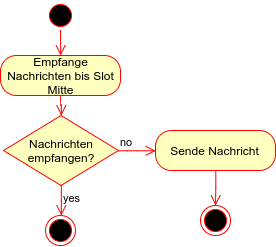
\includegraphics[width=0.4\textwidth]{send-collision.png}
\caption[send-collision]{Sendevorgang mit Kollisionserkennung}
\label{fig:send-collision}
\end{figure}

Wenn vor dem Senden Nachrichten empfangen wurden, dann wird die eigentliche zu sendende Nachricht verworfen und nicht gesendet (siehe Abbildung \ref{fig:send-collision}). Es wird bis zum Ende des Slots gewartet. Die Funktion signalisiert dann, dass nicht gesendet wurde.
Falls vorher keine Nachricht empfangen wurde, wird die Nachricht mit dem nun aktuellen Zeitstempel über den Socket aus dem State versendet. Danach wird gewartet, bis der Slot abgelaufen ist. Die Funktion signalisiert ein erfolgreiches Senden.

Der Lesevorgang prüft in einem bestimmten Zeitfenster (timeout) jede ms, ob eine Nachricht auf dem Socket anliegt. Falls eine Nachricht anliegt, wird diese in die Liste der empfangenen Nachrichten angefügt. Die daraus resultierende Liste enthält alle empfangenen Nachrichten. Wenn diese Liste genau ein Element enthält, wird dieses Element als Nachricht zurück gegeben. Ansonsten wird das leere Element (nil) zurückgegeben. Das ist der Fall, wenn eine Kollision während des Lesens erkannt wurde.

Die Lese- und Sendevorgänge sind so aufgebaut, dass diese über eine anzugebende Laufzeit laufen. Alle Zeitabhängigen Funktionen wie der aktuelle Zeitstempel, die Zeit bis zum Ablaufen eines Slots oder die Mitte des Slots wird bei der Clock-Komponente abgerufen.

Die Konvertierung der Nachrichten in Bytes zum Versend und die Konvertierung der Bytes in Nachrichten beim Empfang geschieht durch das Datagram Modul.

\subsection{Konfigurationsparameter}
\begin{itemize}
	\item Interfacename
	\item Multicastadresse
	\item Port
\end{itemize}

\section{Payload-Source}
\subsection{Aufgabe und Verantwortung}
Die Payloud-Source Komponente ist für das Bereitstellen der zu verwendenden Nutznachrichten zuständig. Diese kommen aus einer externen Datenquelle.

\subsection{Schnittstelle}
\begin{lstlisting}
; Startet die Komponente mit angegebenen Kanal
Kanal -> Komponente
new-payload-source(out-chan)
\end{lstlisting}

\subsection{Entwurfsentscheidungen}
Die Payload-Source Komponente ist ein eigenständiger Prozess. Die Nutzdaten (24 Bytes) werden in diesem Prozess ständig aus dem STDIN gelesen und auf einen Kanal gelegt. Dieser Kanal ist mit der Stations Komponente verbunden. Dadurch werden auf den Kanal alle empfangenen Nutzdaten aus der externen Datenquelle auf diesem Kanal nebenläufig hinzugefügt. Wenn der Kanal eine Größe größer Null hat, dann dient dieser gleichzeitig als Nutzdatenbuffer und hält immer eine bestimmte Anzahl an Nutzdaten bereit.

\subsection{Konfigurationsparameter}
\begin{itemize}
	\item Kanalgröße
\end{itemize}

\section{Message-Writer}
\subsection{Aufgabe und Verantwortung}
Der Message-Writer dafür zuständig empfangene Nachrichten in einer Datei bereit zu stellen.

\subsection{Schnittstelle}
\begin{lstlisting}
; Startet die Komponente mit angegebenen Kanal
Kanal -> Komponente
new-message-writer(in-chan)
\end{lstlisting}

\subsection{Entwurfsentscheidungen}
Der Message-Writer ist ein eigener Prozess, der kontinuierlich eine Nachricht (falls vorhanden) aus dem Kanal herausnimmt und die Nutzdaten aus dieser an eine Datei als neue Zeile anfügt. Der Kanal aus dem entnommen wird kann eine feste Größe haben. Eine Größe größer Null veranlasst, dass der Kanal als Buffer von gelesenen Nachrichten fungiert.

\subsection{Konfigurationsparameter}
\begin{itemize}
	\item Kanalgröße
	\item Ausgabedatei
\end{itemize}

\section{Clock}
\subsection{Aufgabe und Verantwortung}
Die Clock ist der zentrale Anfragepunkt für die aktuellen Zeit und zeitabängige Werte. Dazu gehören die restliche Zeit bis zu einem Slot- oder Frameende, der aktuelle Slot in Abhängigkeit von der Zeit, die restlichen Slots in Abhängigkeit von der Zeit und die Zeit bis zur Mitte eines Slots. Die aktuelle Zeit hat eine einstellbare Abweichung.

\subsection{Schnittstelle}
\begin{lstlisting}
; Enthaelt den State mit der Abweichung
() -> State
offset

; Gibt die aktuelle Zeit + Abweichung zurueck
() -> Nummer
current-time

; Gibt den aktuellen Frame zurueck, abhaengig der Framelaenge
Nummer -> Nummer
current-frame(frame-size)

; Gibt den aktuellen Slot zurueck, abhaengig der Framelaenge und
; Slotanzahl
(Nummer, Nummer) -> Nummer
current-slot(frame-size, slot-count)

; Gibt Anzahl der restlichen Slots im Frame zurueck
(Nummer, Nummer) -> Nummer
remaining-slots(frame-size, slot-count)

; Gibt die restlichen ms pro festen Zeitabstand zurueck
Nummer -> Nummer
remaining-time-until-end(duration)

; Blockiert den aufrufenden Prozess bis ein Slot abgelaufen ist
Nummer -> ()
wait-until-slot-end(slot-duration)

; Zeit bis die Mitte eines Slots erreicht ist
Nummer -> Nummer
ms-until-slot-middle(slot-duration)

; Startet die Komponente mit dem einkommenden Kanal
Kanal -> Komponente
new-clock(in-chan)
\end{lstlisting}

\subsection{Entwurfsentscheidungen}
Die Komponente ist ein eigenständiger Prozess und stellt Funktionen, die in Abhängigkeit zur aktuellen Zeit stehen zur Verfügung. Sie enthält einen State, der die Abweichung speichert. Die Komponente an sich wird nur vom Connector und von der Station verwendet.

Die Clock Komponente verarbeitet in ihrem Prozess die Nachrichten, die im einkommenden Kanal  von der Stationskomponente sind. Die Nachrichten in diesem Kanal enthalten zusätzlich die Zeit, zu der sie angetroffen sind.
Wenn die Nachricht von einer Station der Klasse A kommt, wird sie weiter behandelt. Nachricht von Stationen der Klasse B werden nicht weiter betrachtet.
Anhand der Ankunftszeit und der Sendezeit und dem vorherigen Offset, wird die Abweichung neu berechnet (siehe Gleichung \ref{equ:offset-calculation}).
\begin{equation}
Offset_{i+1} = \frac{Offset_i + (Empfangszeit - Sendezeit)}{2}
\label{equ:offset-calculation}
\end{equation}

\subsection{Konfigurationsparameter}
\begin{itemize}
    \item Anfänglicher Offset
\end{itemize}

\section{Station}
\subsection{Aufgabe und Verantwortung}
Die Station ist für die Verwaltung der Slots und das Koordinieren des sequentielle Senden und Empfangen von Nachrichten verantwortlich. Dabei werden die Nutzdaten des einkommenden Kanals von der Payload-Source Komponente zum Versenden der Nachrichten genommen.
Einkommende Nachrichten werden auf den ausgehenden Kanal zur Message-Writer Komponente gelegt.

\subsection{Schnittstelle}
\begin{lstlisting}
; Startet die Komponente mit den Kanaelen
(Kanal, Kanal, Kanal) -> Komponente
new-station(in-chan, out-chan-clock, out-chan-message-writer)
\end{lstlisting}

\subsection{Entwurfsentscheidungen}
Die Station ist ein eigener Prozess. Sie hat einen State, in dem der aktuelle Slot zum Senden und die Stationsklasse gespeichert ist. Sie benutzt den Connector, um Daten zu senden und zu empfangen. Die Clock Komponente wird verwendet um die jeweiligen Slots und Frames zu identifizieren.

Der Arbeitsablauf der Station besteht aus einer Initalisierungsphase und einer Hauptphase.
Die Initialisierungsphase beginnt damit, alle Nachrichten bis zum Ende des aktuellen Frames $n$ zu lesen und die erhaltenen Nachrichten nach freien Slots und der Zeitsynchronisation auszuwerten.
Die empfangenen Nachrichten erweitert um die jeweiligen Zeit des Empfanges werden auf den ausgehenden Kanal zur Clock Komponente getan. Dort werden Sie dann ausgewertet. Die Empfangenen Nachrichten werden außerdem auf den ausgehenden Kanal zum Message-Writer gelegt.
Freie Slots werden ausgewählt, indem von den 25 verfügbaren Slots die Slots aus den erhaltenen Nachrichten entfernt werden. Dadurch bleiben nur noch die Slots übrig, in denen im nächsten Frame $n + 1$ nicht gesendet wird. Von diesen freien Slots wird ein zufälliger Slot gewählt, den die Station zum Senden im Frame $n + 1$ verwendet und im State speichert.

Nun beginnt die Hauptphase. In der Hauptphase wird bis zum derzeitigen gespeicherten Slot aus dem State gelesen. Die empfangenen Nachrichten werden wieder nach freien Slots für das nächste Frame und für die Zeitsynchronisation ausgewertet (wie in der Initialisierungsphase). Aus den freien Slots wird wieder ein zufälliger gewählt und im State gespeichert. Das ist der Slot zum Senden im nächsten Frame.
Danach fängt die Station an zu senden. Dazu wird ein Nutzdatenpaket aus dem einkommenden Kanal von der Payload-Source Komponente genommen, falls eins vorhanden ist. Wenn keins vorhanden ist, wird nicht gesendet.
Wenn eins vorhanden ist, wird diese an die zu sendende Nachricht hinzugefügt, wie auch die Stationsklasse und der Slot aus dem State (Slot für das Senden im nächsten Frame).
Diese Nachricht wird dann mit dem Connector versendet.
Wenn das Versenden ein Erfolg war (keine Kollision), dann wird bis zum Ende des Frames wieder gelesen. Die dadurch erhaltenen Nachrichten werden wieder zur Zeitsynchronisation auf den ausgehenden Kanal zur Clock Komponente gelegt.
Wenn das Versenden nicht erfolgreich war (Kollision), dann wird wie im erfolgreichen Fall vorgegangen, nur wird zusätzlich am Ende des Frames wieder ein neuer freier Slot zum Senden gewählt (in Abhängigkeit der empfangenen Nachrichten). Dieser Slot wird dann wieder im State gespeichert (siehe Abbildung \ref{fig:station-collision}).
Danach fängt die Hauptphase wieder von vorne an (Schleife).

\begin{figure}[h]
\centering
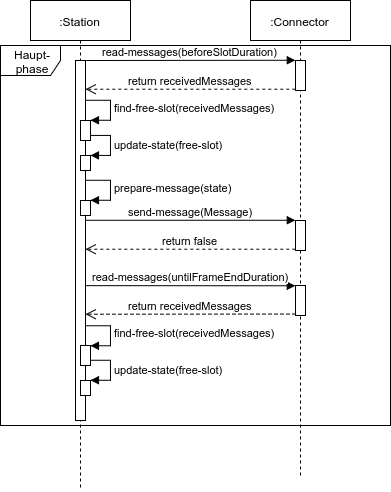
\includegraphics[width=0.4\textwidth]{station-collision.png}
\caption[station-collision]{Kollisionsbehandlung beim Senden}
\label{fig:station-collision}
\end{figure}

\subsection{Konfigurationsparameter}
\begin{itemize}
    \item Stationsklasse
    \item Framegröße
    \item Gesamtanzahl der Slots
\end{itemize}

\chapter{Kollisionsfreier Ablauf}
Es wird ein kollisionsfreier Ablauf in anbetracht von maximal 25 Teilnehmern auf dem Medium angestrebt und näher untersucht.

Die Station stößt in festen Frames sequentiell das Senden und Empfangen an. Kollisionen können hier durch verschiedene Gegebenheiten auftreten.
Zum einen kann ein zeitlicher Versatz vorhanden sein, wodurch nicht in den richtigen Slots empfangen und vor allem gesendet wird. Das wird durch die Auswertung der empfangenen Nachrichten und der Neuberechnung der Abweichung der UTC-Zeit (Zeitsynchronisation) abgefangen.
Die Station muss also darauf achten, ihre sequentielle Arbeit in den Frames einzuhalten und sich immer in den festen Slots im Frame bewegen. Das wird durch den Connector garantiert, dessen Lese- und Sendevorgänge immer mit Timeouts arbeiten. Dadurch kann sich ein kollisionsfreier Ablauf in endlicher Zeit einpendeln.

Eine andere Quelle für Kollisionen kann entstehen, wenn alle Stationen nach einer festen Regel freie Slots auswählen und dadurch die gleichen Slots zum Senden im nächsten Frame haben. Das wird wiederum durch die Stations Komponente umgangen, in dem immer ein zufälliger freier Slot gewählt wird. Dadurch verteilt sich die Slot Auswahl und ein kollisionsfreier Ablauf kann sich mit der Zeit wieder einpendeln.

Zusätzlich dazu werden Kollisionen vermieden, in dem der Connector das Senden auf Kollisionen überprüft und das der Station meldet. Die Station wählt dadurch ja am Ende des Frames eine neue Station zum Senden im nächsten Frame aus den vorhandenen Nachrichten aus, was eine Kollision aktiv verhindert und zum kollisionsfreien Ablauf beiträgt.

Durch diese Maßnahmen kann ein kollisionsfreier Ablauf in endlicher Zeit erreicht werden.

%% appendix if used
%%\appendix
%%\typeout{===== File: appendix}
%%\include{appendix}

% bibliography and other stuff
\backmatter

\typeout{===== Section: literature}
%% read the documentation for customizing the style
\bibliographystyle{dinat}
\bibliography{documentation}

\typeout{===== Section: nomenclature}
%% uncomment if a TOC entry is needed
%%\addcontentsline{toc}{chapter}{Glossar}
\renewcommand{\nomname}{Glossar}
\clearpage
\markboth{\nomname}{\nomname} %% see nomencl doc, page 9, section 4.1
\printnomenclature

%% index
\typeout{===== Section: index}
\printindex
\chapter{Erklärung zur schriftlichen Ausarbeitung des Referates}
\HAWasurency

\end{document}
